\documentclass[a4paper,10pt,fullpage]{article}
\usepackage[utf8]{inputenc}
\usepackage[english]{babel}
\usepackage[a4paper]{geometry}		
\geometry{top=1.5cm, bottom=1cm, left=2cm, right=1.5cm} 	
\usepackage{hyperref}
\usepackage{enumitem}
\usepackage{graphicx}
\usepackage{wrapfig}
%\graphicspath{ {./images/} }
\pagenumbering{gobble}
\setlength{\parindent}{0em}


% % % % % % % % % % % % % % % % % % % % % % % % % % % % % % % % % % % % %
\begin{document}
\setlist{nolistsep}

% % % % % % % % % % % % % % % % % % % % % % % % % % % % % % % % % % % % %

\begin{wrapfigure}{l}{0.21\textwidth}
	%\centering
	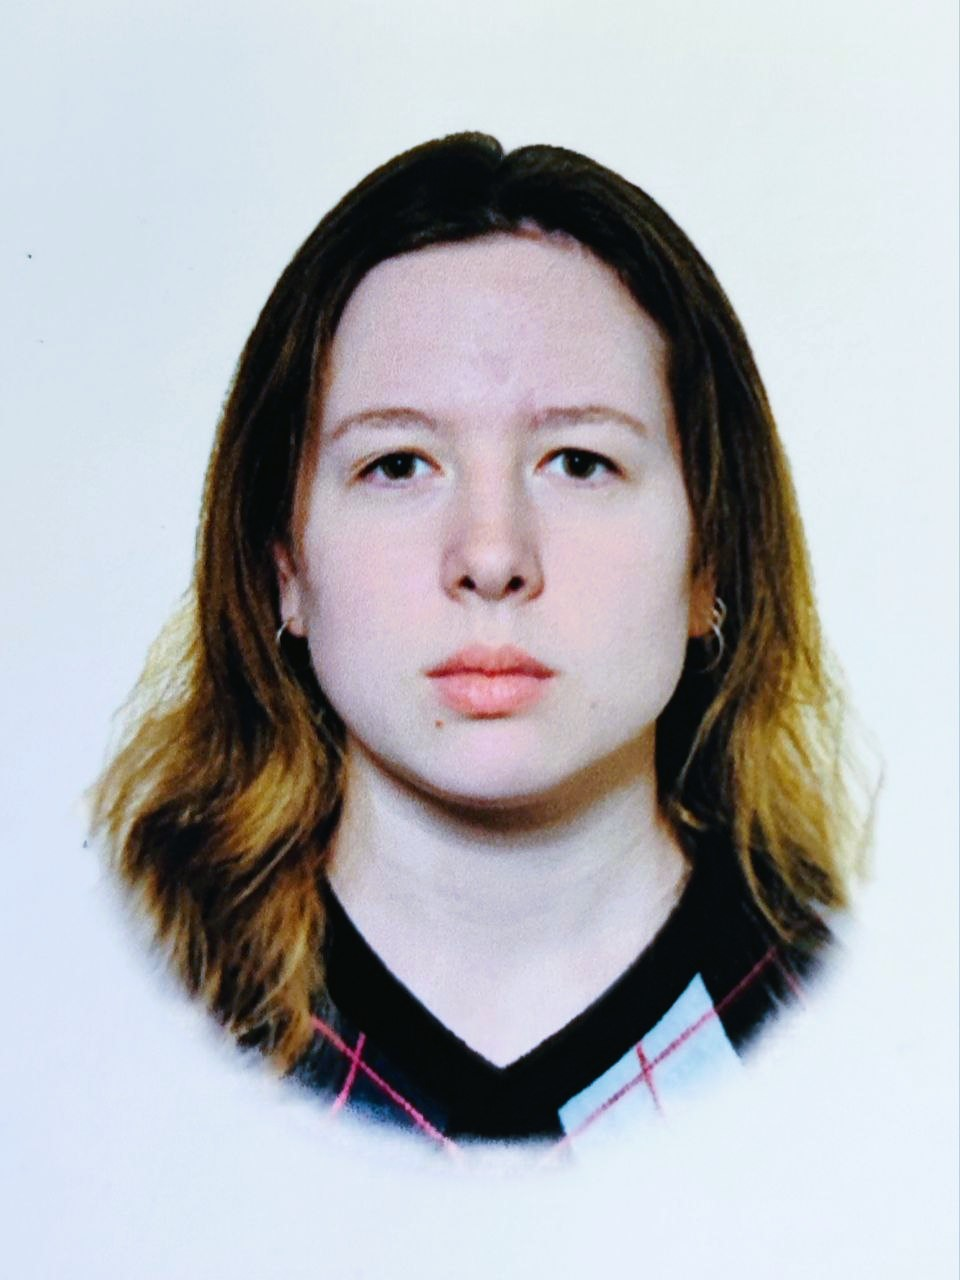
\includegraphics[width=0.21\textwidth]{photo1}
\end{wrapfigure}

%\begin{center}
\underline{\textbf{\LARGE Svetlana Golubeva}}\\
%	\vspace{5pt}
%	{\Large Barista}
%\end{center}

\underline{Contatti:} lana.a.golubeva@gmail.com, Cel: +39 342 7996584, LinkedIn: \href{https://www.linkedin.com/in/lana-golubeva/}{lana-golubeva}. \\
%\underline{LinkedIn:} \href{https://www.linkedin.com/in/lana-golubeva/}{lana-golubeva.}\\
%\underline{Data di nascita:} 26 Ottobre 1989.\\
\underline{Residenza:} Lipomo(CO), Italia. %Eligible to work in Europe.\\


%\underline{GitHub:} \href{https://github.com/attillax}{attillax}\\
%\hline
%\vspace{10pt}

% % % % % % % % % % % % % % % % % % % % % % % % % % % % % % % % % % % % %
\begin{center}
	\underline{\textbf{\large Competenze:}}
\end{center}
\underline{Linguaggi di programmazione}: Python, SQL, R, C.\\
\underline{Metodologie di sviluppo}: Agile, Scrum, Kanban.\\
\underline{Aree di competenza}: Amministrazione delle reti, analisi dei dati, automatizazione dei processi.\\
\underline{OS}: Windows, Linux (Debian, Slackware, LFS).\\
\underline{Altro}: Git, MS Office, \LaTeX, TiKz, UML, BPM, Emacs, Notion, Tableau.\\
\underline{Lingue:} Russo (madrelingua), Italiano (avanzato), Inglese (avanzato), Tedesco (scolastico), Francese (scolastico).%\\
%\hline
%\vspace{10pt}


% % % % % % % % % % % % % % % % % % % % % % % % % % % % % % % % % % % % %
\begin{center}
	\underline{\textbf{\large Esperienza:}}
\end{center}	

\textbf{Como Luxury Suites} Como, Italia (9 mesi).\\
\underline{Receptionist}, Luglio 2023 – ...\\

\textbf{Consulente di Business Intelligence e Analista dei Dati} (5 anni 4 mesi).\\
\underline{Freelance}, Settembre 2017 – Decembre 2022.
\begin{itemize}
	\item[--] Transformazione digitale, automazione e ottimizzazione dei processi aziendali.\\
\end{itemize}

%\textbf{El Merendero} Como, Italia (4 mesi).\\
%\underline{Sala \& Banco}, Maggio 2022 – Agosto 2022.\\

\textbf{A' Design Award \& Competition} Como, Italy (5 anni 3 mesi).\\
\underline{Responsabile della Logistica}, Maggio 2019 - Novembre 2021.
\begin{itemize}
	\item[--] Ottimizzazione dei processi aziendali.	
	\item[--] Gestione del personale sulla linea di produzione.
%	\item[--] Miglioramento della catena di preparazione della merce.
\end{itemize}
\underline{Specialista della Logistica}, Settembre 2017 - Aprile 2019.
\begin{itemize}
	\item[--] Allestimento di mostre di design.
	\item[--] Pianificazione e preparazione di serata di Gala.
	\item[--] Gestione e ottimizzazione dei processi di produzione e di spedizione della merce.
\end{itemize}
\underline{Consulente Tecnico}, Settembre 2016 - Agosto 2017.
\begin{itemize}
	\item[--] Gestione e miglioramento dell'infrastruttura IT.\\
	%	\item[--] Developed, tested and implemented new marketing strategies. \\
\end{itemize}



\textbf{Moscow State Institute of Radio Engineering, Electronics and Automation (MIREA)} Moscow, Russia (6 anni).\\
\underline{Senior Technical Consultant}, Settembre 2015 – Agosto 2017.
\begin{itemize}
%	\item[--] PhD Candidate.
	\item[--] Supervisione e project management per studenti laureati.
	\item[--] Architettura concettuale del sistema di ricerca per il portale del dipartimento.
	\item[--] Integrazione dei metodi ML nelle ricerche scientifiche.
	\item[--] Sviluppo di un concetto per il monitoraggio di attività sospette basato sul comportamento degli utenti nelle reti IoT.
\end{itemize}
\underline{Technical Consultant}, Settembre 2013 – Agosto 2015.
\begin{itemize}
	\item[--] Sviluppo della proposta di trasferimento dell'infrastruttura dipartimentale da proprietario a open source
	Software.
	\item[--] Partecipazione allo sviluppo dell'architettura per il portale didattico e amministrativo del dipartimento.
	\item[--] Strutturazione e aggiornamento dei corsi didattici per il dipartimento.
\end{itemize}
\underline{System Administrator}, Settembre 2011 – Agosto 2013.
\begin{itemize}
	\item[--] Gestione della rete del dipartimento e dei laboratori informatici.
	\item[--] Assistenza didattica ai professori.
\end{itemize}

%\hline
%\vspace{10pt}
% % % % % % % % % % % % % % % % % % % % % % % % % % % % % % % % % % % % %
\begin{center}
	\underline{\textbf{\large Formazione scolastica:}}
\end{center}	
\textbf{Politecnico di Milano}, Como, Italia.\\
2013 - 2016 --- Corsi magistrali in Ingeneria Informatica (programma di scambio academico, doppia laurea.)\\

\textbf{Moscow State Institute of Radio Engineering, Electronics and Automation (MIREA)}, Mosca,
Russia.\\
2013 - 2015 --- M.Sc. in Ingeneria Informatica.\\
2011 - 2013 --- Traduttore di area di attività professionale. \\
2009 - 2013 --- B.Sc. in Ingeneria Informatica.


%\hline
%\vspace{10pt}
% % % % % % % % % % % % % % % % % % % % % % % % % % % % % % % % % % % % %
\begin{center}
\underline{\textbf{\large Certificati:}}
\end{center}	

\textbf{Stanford University}, Lagunita MOOC.\\
2016 --- Statistical Learning.

%\hline
%\vspace{10pt}
% % % % % % % % % % % % % % % % % % % % % % % % % % % % % % % % % % % % %
%\begin{center}
%\underline{\textbf{\large Languages:}}
%\end{center}		
	
%\underline{Russian}: native, \underline{English}: advanced, \underline{Italian}: upper-intermediate.\\


% % % % % % % % % % % % % % % % % % % % % % % % % % % % % % % % % % % % %


% % % % % % % % % % % % % % % % % % % % % % % % % % % % % % % % % % % % %
\vfill
%Como, Italy

\hline
\vspace{3pt}
\scriptsize Autorizzo il trattamento dei miei dati personali presenti nel curriculum vitae ai sensi del Decreto Legislativo 30 giugno 2003, n. 196 e del GDPR (Regolamento UE 2016/679).

% % % % % % % % % % % % % % % % % % % % % % % % % % % % % % % % % % % % %
\end{document}
